\documentclass{article}
\usepackage[utf8]{inputenc}
\usepackage[margin=2cm]{geometry}
\usepackage{amsmath}
\usepackage{amssymb}
\usepackage{amsthm}
\usepackage{graphicx}
\usepackage{subfig}
\usepackage{enumitem}

\title{Conditional SMC genealogies}
\author{Suzie Brown\\ {\small supervised by Adam Johansen, Jere Koskela, Paul Jenkins \& Dario Span\`o}}
\date{\today}

%\usepackage[colorlinks=true, allcolors=blue]{hyperref}
\usepackage[round, sort&compress]{natbib}
\usepackage{har2nat} %%% Harvard reference style
\bibliographystyle{agsm}

\newcommand{\E}{\mathbb{E}}
\newcommand{\PR}{\mathbb{P}}
\newcommand{\V}{\operatorname{Var}}
\newcommand{\vt}[2][t]{v_{#1}^{(#2)}}
\newcommand{\vttilde}[2][t]{\tilde{v}_{#1}^{(#2)}}
\newcommand{\wt}[2][t]{w_{#1}^{(#2)}}
\newcommand{\eqdist}{\overset{d}{=}}
\newcommand{\Bin}{\operatorname{Bin}}
\newcommand{\N}{\mathcal{N}}
\newtheorem{thm}{Theorem}

\begin{document}
\maketitle

\section{Introduction}

\section{Background}
The Wright-Fisher model \citep[Chapter 3]{wakeley2009}, popular in the analysis of population genetics, includes some simplifying assumptions that make it somewhat unrealistic for that application. Namely, it is assumed that the population size is constant, and that generations do not overlap. 
While these constraints may hamper the model's applicability to population genetics, it is pleasing to note that when re-purposed for the analysis of SMC genealogies, both of these rather restrictive assumptions apply automatically. At least in the most common SMC algorithms, the number of particles (population size) remains constant at each iteration, and the resampling (reproduction) procedure is applied to all particles at once.

However, a significant alteration must be made to the standard Wright-Fisher model before it can be applied to SMC. The offspring distributions of each particle are not exchangeable, because broadly speaking, offspring of parents with high weight will tend to have high weight themselves. This follows intuitively from the notion that propagating a particle from a high density region at time $t$ will result in a new state that is close to the high density region at time $t+1$.

There are generalisations of the Wright-Fisher model that do not require exchangeability among individuals, since it is also an important feature in population models. For instance, it can incorporate the existence of a hereditary trait whose value affects fertility. To model SMC genealogies, it is necessary to go one step further by allowing dependence between offspring distributions at different generations. This alteration amounts to a significant qualitative change since, while the forward process is still Markovian, the reverse (coalescent) process is not.

Whilst the population genetics literature has typically focused on the proliferation of hereditary traits \citep[Chapter 3]{wakeley2009}, our interest lies only with the genealogical process itself. The advancement of the trait, say ``being in a high density region'' is taken care of in the construction of the SMC algorithm. However, it is well-known that the problem of ``ancestral degeneracy'' is the source of much pain for practitioners; hence our interest in quantifying this problem.

\subsection{Previous work}
Kingman \citep{kingman1982gene, kingman1982coal, kingman1982exch} studied the asymptotic properties of the genealogies arising in a number of exchangeable population models, including the standard Wright-Fisher model. He showed that they each converge in the limit $N\to\infty$ (with appropriate time rescaling) to a Markov process termed the $n$-coalescent. By studying this limiting process, he was able to establish some new results about the behaviour of such populations, and produce novel derivations of some known results.

\citet{mohle1998} extends this result to a class of non-exchangeable models, with the assumption that offspring distributions are independent between different generations. This allows application to more complex population models; but is still too restrictive to cover SMC genealogies, which by construction have strong dependence between generations.

Allowing for dependence between generations significantly complicates the computations, because the coalescent process is no longer Markovian. \citet{koskela2018} addresses a first case of such models, applicable to a range of standard SMC procedures, under some reasonable conditions.

We would like to extend to the case of conditional SMC, which differs substantially from the case of \citet{koskela2018} because there is a particular ancestral line that is conditioned to survive. This extension is important to make the results applicable to the particle Gibbs algorithm \citep{andrieu2010}, which is popular across a range of applications.

\subsection{Sequential Monte Carlo}

\subsubsection{Conditional SMC}

%\subsection{Population genetics}
%The Wright-Fisher model, popular in the analysis of population genetics, bears some simplifying assumptions that render it unrealistic for that application. Namely, the population size is assumed to remain constant, and the generations non-overlapping. While these constraints may hamper the model's applicability to population genetics, it is pleasing to note that when re-purposed for the analysis of SMC genealogies, both of these rather restrictive assumptions apply automatically. At least in the most common SMC algorithms, the number of particles (population size) remains constant at each iteration, and the resampling (reproduction) procedure is applied to all particles at once.
%
%It seems then that the myriad tools and results developed for this model by population geneticists should be seamlessly transferable to the analysis of SMC genealogies. In reality, a significant alteration must be made to the standard Wright-Fisher model before it can be of use in this context: the offspring distributions of each particle are not exchangeable, because broadly speaking, offspring of parents with high weight will tend to have high weight themselves. This follows intuitively from the notion that propagating a particle from a high density region at time $t$ will result in a new state that is close to the high density region at time $t+1$.
%
%This effect can naturally be interpreted in the population genetics framework as the existence of a hereditary trait whose value affects fertility. A typical and well-studied question in the population genetics literature addresses the proliferation of such a trait \citep[Chapter 3]{wakeley2009}. For example, in the Wright-Fisher model it is possible to study the dynamics of the proportion of the population having the trait of interest, ultimately in the limit as the number of generations goes to infinity. However, the question of how prevalent the ``high density'' trait may be in our population of particles is tangential to our focus (the resampling step is constructed in such a way as to maintain the desired dynamics, i.e.\ consistent estimation of the target distribution). Our interests lie instead with the genealogy of the particles, regardless of the properties they thus inherit.




\section{Theoretical results}
We now consider extending the results of \citet{koskela2018} to the case of conditional SMC.
In particular, the SMC updates will be conditioned on a particular trajectory surviving. We concentrate on the exchangeable model, so we may take WLOG that the ``immortal line'' is the trajectory containing individual 1 from each generation.
We first assume the simplest case, with multinomial resampling; analogous to the standard SMC case where
\begin{equation*}
\vt{i} \eqdist \Bin (N, \wt{i}), \qquad i=1,\dots,N
\end{equation*}
yielding the coalescence rate
\begin{equation}
c_N(t) := \frac{1}{(N)_2} \sum_{i=1}^{N} \E\left[ (\vt{i})_2 \right] = \sum_{i=1}^{N} \E\left[(\wt{i})^2\right].
\end{equation}
But now, since the first line is immortal, in each time step the first individual must have at least one offspring. The remaining $N-1$ offspring are assigned multinomially to the $N$ possible parents as usual, giving the offspring numbers:
\begin{align*}
& \vttilde{1} \eqdist 1 + \Bin(N-1, \wt{1}) \\
& \vttilde{i} \eqdist \Bin(N-1, \wt{i}), \qquad i=2,\dots,N.
\end{align*}
We therefore have the following moments (using tower property):
\begin{align*}
& \E[\vttilde{i}] = (N-1)\E[\wt{i}] &\\
& \E[(\vttilde{i})^2] = (N-1)(N-2)\E[(\wt{i})^2] + (N-1)\E[\wt{i}] &\qquad i=2,\dots,N \\
& \E[\vttilde{1}] = (N-1)\E[\wt{1}] + 1 \\
& \E[(\vttilde{1})^2] = (N-1)(N-2)\E[(\wt{1})^2] + 3(N-1)\E[\wt{1}] + 1 &
\end{align*}
and we can derive the altered coalescence rate:
\begin{align}
\tilde{c}_N(t) &= \frac{1}{(N)_2} \sum_{i=1}^{N} \E\left[ (\vttilde{i})_2 \right] \notag\\
&= \frac{1}{(N)_2} \E\left[ (\vttilde{1})^2 - \vttilde{1} \right] + \frac{1}{(N)_2}\sum_{i=2}^{N} \E\left[ (\vttilde{i})^2 - \vttilde{i} \right] \notag\\
&= \frac{1}{(N)_2}\left[ (N-1)(N-2)\E[(\wt{1})^2] + 2(N-1)\E[\wt{1}] \right] + \frac{1}{(N)_2} \sum_{i=2}^{N} (N-1)(N-2)\E[(\wt{i})^2] \notag\\
&= \frac{1}{(N)_2} \sum_{i=1}^{N} (N-1)(N-2)\E[(\wt{i})^2] + \frac{1}{(N)_2} 2(N-1)\E[\wt{1}] \notag\\
&= \frac{N-2}{N} c_N(t) + \frac{2}{N} \E[\wt{1}]
%&\overset{N\to\infty}{\longrightarrow} c_N(t) \notag
\end{align}
%Since $\wt{1} \leq 1$ for all $t$, as $N\to\infty$ we have
%\begin{equation*}
%\tilde{c}_N(t) - c_N(t) = O(N^{-1}).
%\end{equation*}
Under the conditions of \citet[Corollary 2]{koskela2018}, we have that $\E[\wt{1}] = O(N^{-1})$, and hence
\begin{equation*}
\tilde{c}_N(t) - c_N(t) = O(N^{-2}).
\end{equation*}
%\begin{equation*}
%\tilde{c}_N(t) = \frac{N-2}{N} c_N(t) + O(N^{-2}) = c_N(t) + O \left( \frac{c_N(t)}{N} \right)
%\end{equation*}
\citet{koskela2018} gives the following bounds on $c_N(t)$:
\begin{equation*}
\frac{C_*}{N-1} \leq c_N(t) \leq \frac{C}{N-1}
\end{equation*}
Then, since $\tilde{c}_N(t)$ differs from $c_N(t)$ by $O(N^{-2})$, for sufficiently large $N$ there exist constants $\tilde{C}, \tilde{C}_*$ such that
\begin{equation*}
\frac{\tilde{C}_*}{N-1} \leq \tilde{c}_N(t) \leq \frac{\tilde{C}}{N-1}
\end{equation*}
and we can thus derive bounds analogous to \citet[(5)-(6)]{koskela2018}:
\begin{align}
\frac{N-1}{\tilde{C}_*}t &\leq \tilde{\tau}_N(t) \leq \frac{N-1}{\tilde{C}}t \label{eq:tau_bounds1}\\
\frac{N-1}{\tilde{C}_*}(s-t) &\leq \tilde{\tau}_N(s) - \tilde{\tau}_N(t) \leq \frac{N-1}{\tilde{C}}(s-t) \label{eq:tau_bounds2}
\end{align}
Furthermore, we have that
\begin{align*}
\frac{\tilde{C}}{N-1} &= \frac{N-2}{N} \frac{C}{N-1} + O(N^{-2}) \\
&= \frac{C}{N-1} + O(N^{-2})
\end{align*}
therefore $\tilde{C} - C = O(N^{-1})$ and similarly $\tilde{C}_* - C_* = O(N^{-1})$. Hence the bounds in \eqref{eq:tau_bounds1}, \eqref{eq:tau_bounds2} are asymptotically equal to those of \citet[(5)--(6)]{koskela2018}.

It remains to verify that the conditions \citep[(3)--(4)]{koskela2018} can extend to this case. If so, a modified version of \citet[Theorem 1]{koskela2018} and its corollaries will hold, by the same argument, for conditional SMC.

\section{Simulation study}
In order to investigate how well the asymptotic results hold for finite $N$, we conducted a simulation study on the Ornstein-Uhlenbeck model, a ``simplest case'' hidden Markov model which is popular for such studies in the literature:
\begin{align*}
& X_0 \sim \N(0,1) \\
& X_{t+1} \mid X_t \sim \N((1-\Delta)X_t, \Delta) \\
& Y_t \mid X_{t} \sim \N(X_t, \sigma^2)
\end{align*}
with parameters $\Delta >0, \sigma >0$.

Tree height $T$ is one of the basic properties of an ancestral sub-tree. It denotes the number of generations back one must go to find the most recent common ancestor (MRCA) of a sample of $n$ leaves (individuals from generation $N_{obs}$). That is, how many time steps of the reverse process pass before the $n$ sampled lineages all coalesce to a single lineage. If the asymptotic genealogical process is known to be an $n$-coalescent, moments of $T$ are available analytically. In particular, we expect for conditional SMC to obtain the same limiting process as for standard SMC, since we have shown in Section [REF] that their coalescent rates are asymptotically equal. Therefore in the limit as $N\to\infty$ we expect the moments of $T$ to behave as stated in \citet[Corollary 1]{koskela2018}:
\begin{align*}
\frac{C_*}{C^2} \left(1-\frac{1}{n}\right) + O(N^{-1}) &\leq \E[T/N] \leq 2\frac{C}{C_*^2} \left(1-\frac{1}{n}\right) \\
\left(\frac{4\pi^2}{3} - 12 + O(n^{-1})\right) \left(\frac{C_*}{C^2}\right)^2 + O(N^{-1}) &\leq \V(T/N) \leq \left(\frac{4\pi^2}{3} - 12 + O(n^{-1})\right) \left(\frac{C}{C_*^2}\right)^2
\end{align*}
where of course $T$ depends on $n$ and $N$. In particular, the choice of immortal line does not feature in these bounds and so should have no effect as $N \to\infty$ with respect to $n$.

Following \citet{koskela2018}, we take $\Delta = \sigma = 0.1$ and generate one fixed sequence of observations for use in all SMC runs.
We use a range of values $\{256, 512, \dots, 4096\}$ for $N$, and two fixed values $n=2,16$ intended to show the qualitative difference in behaviour as we cross a supposed ``$n<<N$'' threshold.
The number of observations $N_{obs}$ is taken such that, for all the choices of $n$ and $N$, the $N_{obs}$ generations of SMC particles are enough for the $n$ sampled lineages to coalesce to one common ancestor (with high enough probability that it happens reliably on every repetition); ensuring that the tree height can always be recorded.

For this toy model, the smoothing distribution is available analytically through the Rauch-Tung-Striebel (RTS) smoother \citep{rauch1965}. We exploited this solution to choose the ``immortal line'' on which to condition the conditional SMC updates. Because both the MAP estimate (equal to the mean since the distributions are Gaussian) and variance are available via the RTS smoother, we were able to produce a sequence of immortal lines of decreasing likelihood, by adding multiples of the standard deviation to the mean.

We hypothesised that when $N$ is not too much bigger than $n$, an ``unlikely'' choice of the immortal line should produce qualitative differences in the tree height profile; because the$n$ lineages would often coalesce to the immortal line, which corresponds to an unlikely choice of ancestors under the unconditional algorithm. On the other hand, when $N$ is very large with respect to $n$, this effect should become less significant because the sampled lineages should usually coalesce before interacting with the immortal line.

Figures \ref{fig:kalman_n16} and \ref{fig:kalman_n2} illustrate this distinction. Here we use a decrease in $n$ as a proxy for increasing $N$: over the same range of values for $N$, Figure \ref{fig:kalman_n16} shows the profile for sample size $n=16$, and Figure \ref{fig:kalman_n2} for $n=2$.
We see clearly that in the case of $n=16$, the likelihood of the immortal line significantly affects the tree height profile, while for $n=2$ it makes no appreciable difference.

In any case the mean tree height seems to be higher for conditional SMC (around 0.3) compared to standard SMC (around 0.2), although it is not yet entirely clear.

\begin{figure}
\centering
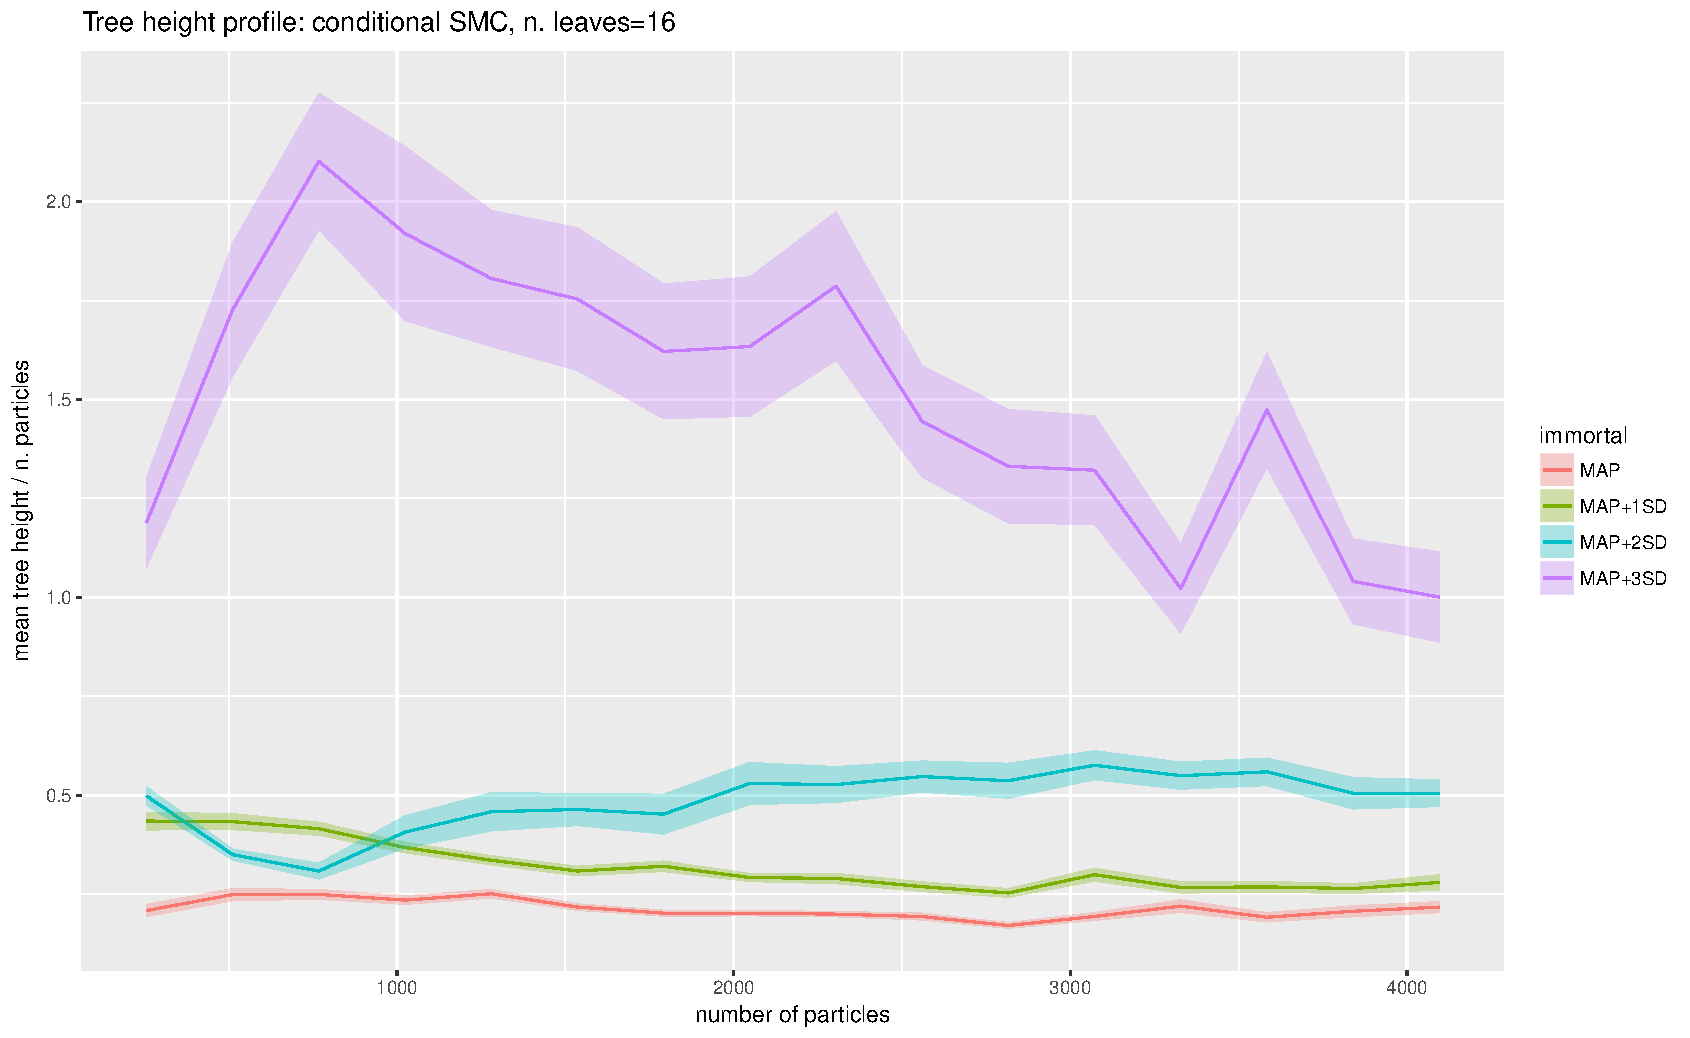
\includegraphics[width=\textwidth]{kalman_n16_100reps_line.pdf}
\caption{$\E(T/N)$ for samples of $n=16$ leaves from conditional SMC where the immortal line is 0,1,2,3 standard deviations away from the MAP estimate. Each point is averaged over 100 repetitions of running the particle filter and sampling $n$ leaves; and the same sequence of observations was used for every run. Different choices of immortal line clearly have a profound effect on tree height: in the number of generations taken for 16 lineages to coalesce, it is likely that the subtree will contain part of the immortal line.}
\label{fig:kalman_n16}
\end{figure}
\begin{figure}
\centering
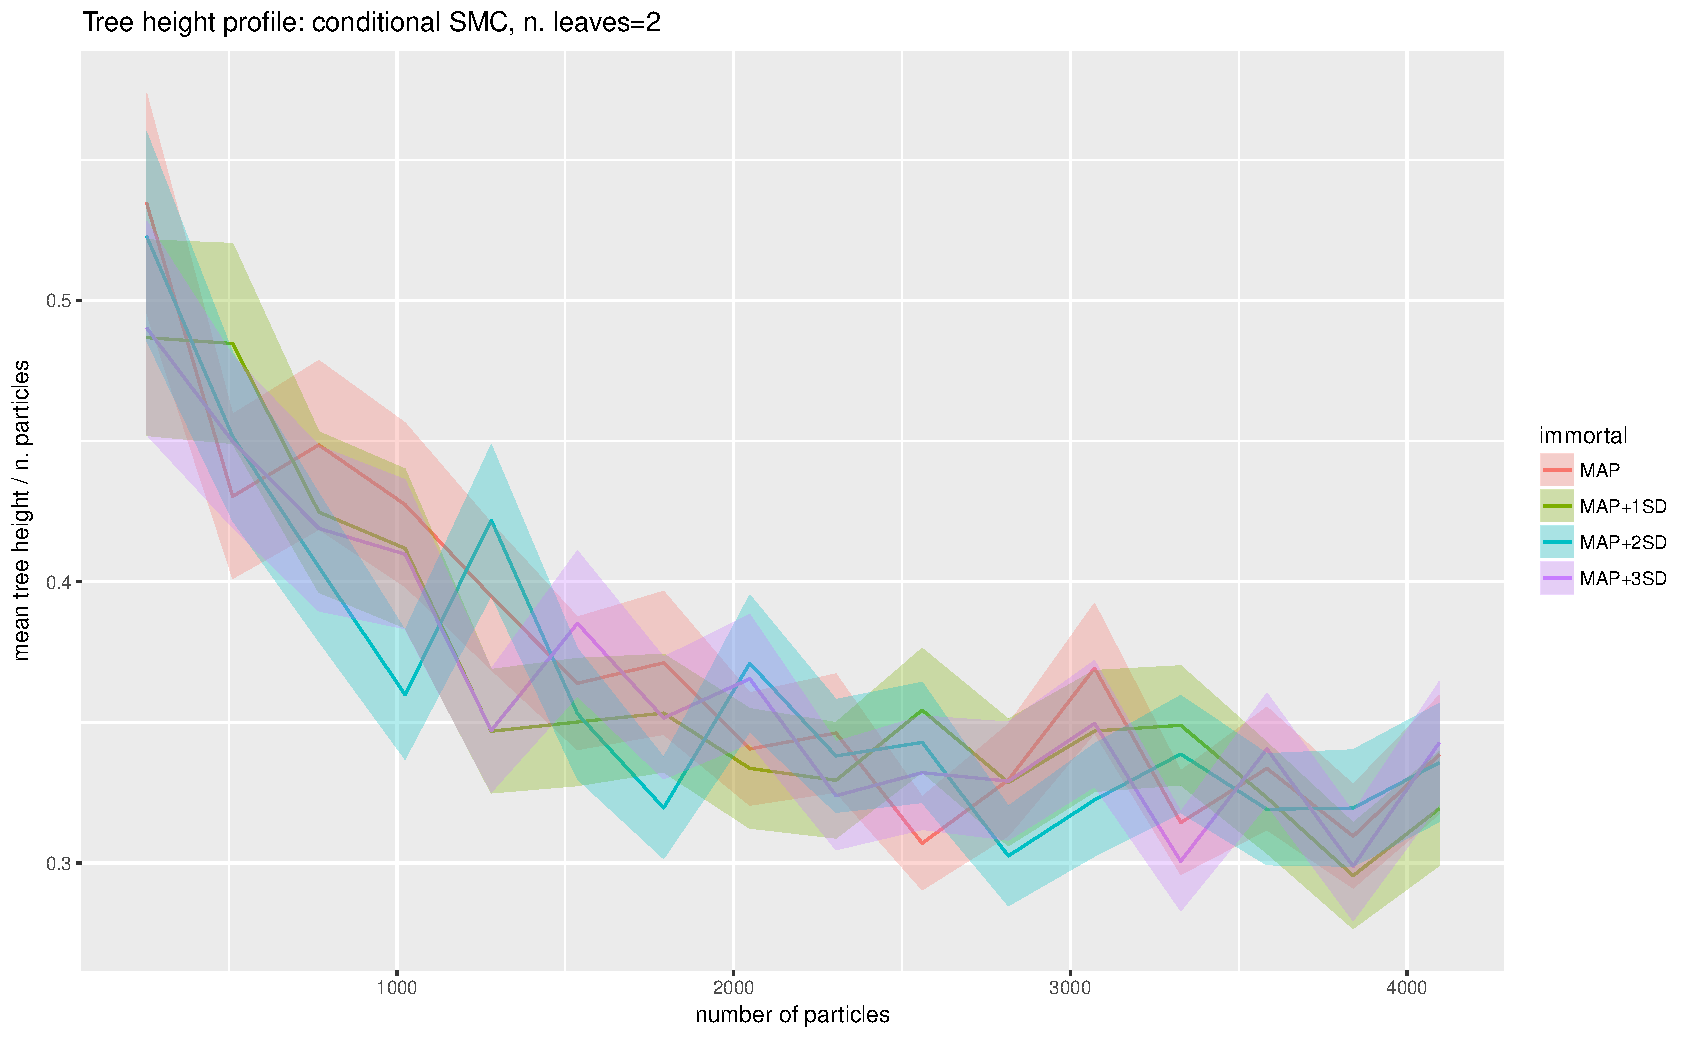
\includegraphics[width=\textwidth]{kalman_n2_1000reps_line.pdf}
\caption{$\E(T/N)$ for samples of $n=2$ leaves from conditional SMC where the immortal line is 0,1,2,3 standard deviations away from the MAP estimate. Each point is averaged over 1000 repetitions of running the particle filter and sampling $n$ leaves; and the same sequence of observations was used for every run. Now the choice of immortal line does not seem to affect the tree height: $n$ is so small compared to $N$  that it is unlikely to sample a pair of lineages that meet the immortal line before coalescing.}
\label{fig:kalman_n2}
\end{figure}

\section{Conclusions}
We have showed that under multinomial resampling, the coalescence probability for conditional SMC is close enough to that of standard SMC to imply the existence of a time rescaling that is asymptotically equivalent to that defined in \citet[p.7]{koskela2018}. Given this result, we expect their result to be transferable to the conditional SMC setting, although conditions \citet[(3)--(4)]{koskela2018} still need to be verified.

While \citet[Section 3]{koskela2018} demonstrates that in the case of standard SMC, the asymptotic results seem to hold even for $n=N$, we conclude from the simulation study that the asymptotic results for conditional SMC will require $n << N$.
Although we have demonstrated empirically that $n <<N$ is required to mitigate the effect of choosing an unlikely immortal line, this in itself should not raise concerns with those implementing the particle Gibbs algorithm. In particle Gibbs, the immortal line is sampled from the trajectories generated in the previous iteration, proportionally to their likelihood. Unless all the generated trajectories are unlikely (in which case there are more profound problems with the algorithm), the immortal line will therefore usually be a reasonably likely one.

We expect that less straight-forward conditional SMC algorithms, using alternative resampling schemes, should have the same limiting genealogical process (up to constants) as the multinomial scheme; as was hypothesised and demonstrated empirically in \citet{koskela2018} for standard SMC. Proving this even for standard SMC remains an open problem.
There are many other directions for generalising these results, in particular investigating their robustness under violation of the various assumptions, either theoretically or empirically. It is of particular interest to consider the classes of SMC algorithms most often used in practice. It was to this end that we began looking at conditional SMC, since the particle Gibbs algorithm is widely used in numerous applications.

\bibliography{smc.bib}
\end{document}